\chapter{How to Speak with Meaning}

Whether we memorize a script, read from one, use a few notes, or use none at all, the lecture insists on a prior point: a talk that is well prepared and passionately delivered can still move an audience. That opening is not a casual encouragement. It clears away the false issue of script format and redirects us to the real problem. What does live delivery add to words that already exist on the page? The answer unfolds step by step. A talk matters because it adds a human layer to information, and that layer must be organized through two variables we can actually control: voice and body.

\section{Why Not Just Email the Script?}

The lecture begins by turning the entire subject into a sharp practical question. If the words are already written, why should we stand in front of a room and say them? Why not simply email the script to everyone who might listen?

This is the right opening question because it refuses to let speaking hide behind ceremony. If the live talk contributes nothing essential, then the live talk is an expensive redundancy. The lecturer therefore puts pressure on the medium itself. What is the spoken event doing that the written page cannot do?

The first contrast can be stated schematically:
\begin{equation}
\text{printed words alone} \neq \text{live talk with human layer}.
\end{equation}

\subsection{Question \& Answer}

\paragraph{Question.} If the words are already written, why give a talk instead of sending the text?

\paragraph{Answer.} Because the talk is not merely a delivery channel for sentences. In live speech, the audience receives not only information but also the speaker's presence. A voice and a body can alter attention, emphasis, trust, urgency, and emotional uptake in ways that a page by itself cannot.

The opening slide records this transmission problem in deliberately stripped-down form. One center addresses many listeners:
\begin{equation}
\text{speaker/message} \longrightarrow \text{audience members}.
\end{equation}

\begin{figure}[h]
\centering

\includegraphics[width=0.58\textwidth]{how_to_speak_with_meaning_figure_02.png}
\end{figure}

\begin{figure}[h]
\centering
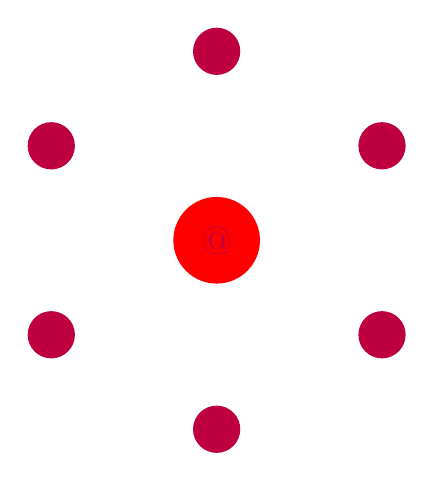
\begin{tikzpicture}[scale=1.0]
\fill[red] (0,0) circle (0.55);
\node[color=purple] at (0,0) {\Large @};

\fill[purple] (0,2.4) circle (0.30);
\fill[purple] (2.1,1.2) circle (0.30);
\fill[purple] (2.1,-1.2) circle (0.30);
\fill[purple] (0,-2.4) circle (0.30);
\fill[purple] (-2.1,-1.2) circle (0.30);
\fill[purple] (-2.1,1.2) circle (0.30);
\end{tikzpicture}
\end{figure}

The slide itself is abstract. It does not yet answer the question. It simply fixes the geometry of the problem: if the message can be distributed from the center outward, what is the necessity of performance? The lecture's next move is to answer that not by metaphor, but by effects.

\section{Humanity Turns Information into Inspiration}

The lecturer says that talks can offer something more than printed words, but that this ``something extra'' does not happen automatically. It has to be thought about, invested in, developed, earned. That insistence matters. The human layer is not guaranteed merely because a person is present onstage. It becomes effective only when it changes what happens inside the listener.

What does that change look like? The lecture answers in the audience's own imagined voice:
\begin{itemize}
\item ``I trust this person.''
\item ``Every sentence sounds interesting.''
\item ``I hear it in your voice and see it in your face.''
\item ``The emphasis on that word with that hand gesture --- now I get it.''
\item ``I can tell how much that hurt you.''
\item ``That passion is infectious.''
\item ``Such determination in those eyes.''
\item ``I want to be on your team.''
\end{itemize}

This sequence is carefully staged. Trust, interest, emphasis, empathy, excitement, conviction, and action are not separate ornaments. They are successive ways in which information becomes active in another mind.

\subsection{Question \& Answer}

\paragraph{Question.} What is the ``something extra'' that a live talk adds beyond the script?

\paragraph{Answer.} It is our humanity, understood operationally: the audible and visible layer that changes how the audience receives the same information. A talk becomes more than text when the speaker's presence turns meaning into something felt, trusted, and acted upon.

The lecture compresses that whole chain into one governing word:
\begin{equation}
\text{humanity} + \text{information} \Longrightarrow \text{inspiration}.
\end{equation}

\begin{definition}
In this lecture, \emph{inspiration} is the force that tells the mind what to do with a new idea instead of allowing that idea to be filed away and forgotten.
\end{definition}

This gives us a clean contrast:
\begin{align}
\text{ordinary idea} &\Longrightarrow \text{filed away}, \\
\text{inspiration} &\Longrightarrow \text{attention alert}.
\end{align}

That transition is the real hinge of the lecture. We begin with a social question about speaking versus writing, but we are now brought to a functional definition. Once inspiration has been defined in terms of what it does, the lecturer can finally ask what variables in the speaker control it.

\section{Two Major Things to Consider}

At this point the lecture pivots from effect to method. If inspiration is the goal, what are the principal things we can work on when preparing a talk? The answer is strikingly economical: there are two major things to consider. What are we doing with the voice? And what are we doing with the body?

This decomposition matters because it prevents the discussion from dissolving into general advice. The lecture does not tell us to ``be charismatic'' or ``be passionate.'' It reduces the field to two controllable variables and then studies them one at a time.

\subsection{Question \& Answer}

\paragraph{Question.} What are the two major things we should actually optimize when preparing a talk?

\paragraph{Answer.} We should optimize two things: the voice, because it shapes how meaning is heard, and the body, because it shapes how confidence, emphasis, and calm are seen.

The structural split may be written as
\begin{equation}
\text{talk preparation} \Longrightarrow \text{voice} + \text{body}.
\end{equation}

The corresponding slide presents this not as a labeled theorem but as a branching form: a large question at the top, a decision point in the middle, and contrasted paths below.

\begin{figure}[h]
\centering

\includegraphics[width=0.68\textwidth]{how_to_speak_with_meaning_figure_03.png}
\end{figure}

\begin{figure}[h]
\centering
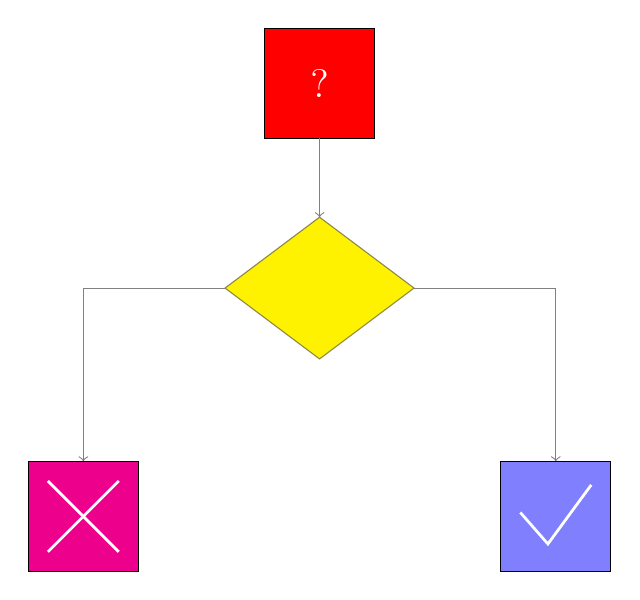
\begin{tikzpicture}[scale=1.0]
\draw[fill=red] (-0.7,2.4) rectangle (0.7,3.8);
\node[color=white] at (0,3.1) {\Large ?};

\draw[->, gray] (0,2.4) -- (0,1.4);

\draw[fill=yellow, draw=yellow!50!black] (0,1.4) -- (-1.2,0.5) -- (0,-0.4) -- (1.2,0.5) -- cycle;

\draw[gray] (-1.2,0.5) -- (-3.0,0.5) -- (-3.0,-1.0);
\draw[gray] (1.2,0.5) -- (3.0,0.5) -- (3.0,-1.0);
\draw[->, gray] (-3.0,-1.0) -- (-3.0,-1.7);
\draw[->, gray] (3.0,-1.0) -- (3.0,-1.7);

\draw[fill=magenta] (-3.7,-3.1) rectangle (-2.3,-1.7);
\draw[white, line width=1pt] (-3.45,-2.85) -- (-2.55,-1.95);
\draw[white, line width=1pt] (-3.45,-1.95) -- (-2.55,-2.85);

\draw[fill=blue!50] (2.3,-3.1) rectangle (3.7,-1.7);
\draw[white, line width=1pt] (2.55,-2.35) -- (2.9,-2.75) -- (3.45,-2.0);
\end{tikzpicture}
\end{figure}

The image is more abstract than the transcript. The transcript resolves the structure by naming the two branches. That order is worth preserving on the page. We first see the form of the split, and then we are told what fills it.

\section{Voice: Variety Based on Meaning}

The lecturer enters the first branch, voice, by example rather than by rule. We are sent to the opening minute of George Monbiot and asked to notice the effect before we are told how the effect is produced. This is pedagogically important. We hear the phenomenon first. Only after that do we name its mechanism.

The exact details of Monbiot's anecdote are not the point here, and the transcript in that region is slightly garbled in places. What matters is the stable lesson surrounding it. His voice adds meaning to every word. The audience feels pulled into his world not simply because the words are good, but because the delivery makes distinctions among them. Some phrases broaden. Some phrases tighten. Some thoughts are allowed to land. We hear structure rather than sequence alone.

\subsection{Question \& Answer}

\paragraph{Question.} How does a speaker make words feel alive rather than merely correct?

\paragraph{Answer.} By creating variety in the way he speaks, and by making that variety answer to meaning. Good vocal variety is not decorative. It is semantic. It tells the audience what carries weight.

The governing rule is therefore
\begin{equation}
\text{variety in speech} \Longrightarrow \text{meaning made audible}.
\end{equation}

The lecture then sharpens the point with a counterexample. Not every talk offers the extra human layer. Some talks flatten themselves. Every sentence receives the same contour, the same small rise and drop, the same pace, the same pressure. The audience is then given a false signal:
\begin{equation}
\text{every sentence sounds the same} \Longrightarrow \text{no part seems more important than any other}.
\end{equation}

That is why the lecture compares such speaking to hypnosis in the bad sense: it lulls the audience to sleep. The problem is not merely boredom. The problem is structural. A uniform voice denies hierarchy to the argument.

\section{Marking the Script So the Voice Can Move}

Once that diagnosis has been made, the lecture becomes procedural. If the talk is scripted, we are told not to wait passively for vocal variation to appear. We should build the variation into the page. In effect, we write a notation for delivery on top of the script.

This is one of the strongest moments in the lecture because it replaces vague advice with a workable algorithm. We begin locally, sentence by sentence, and then move globally, paragraph by paragraph.

\subsection{Question \& Answer}

\paragraph{Question.} How can a scripted talk be marked so that the voice varies with meaning instead of slipping into monotone?

\paragraph{Answer.} We first underline the most important two or three words in each sentence. Then we look for the one word in each paragraph that really matters and underline it twice. After that we add special marks for special local effects: playfulness, questions, jokes, and the main aha moment.

The lecture's notation begins with a distinction between sentence-level and paragraph-level emphasis:
\begin{align}
\text{sentence} &\mapsto \underline{\text{important words}}, \\
\text{paragraph} &\mapsto \underline{\underline{\text{one governing word}}}.
\end{align}

The visual slide records precisely this structure: text-like blocks, and within them, selected positions marked out for emphasis.

\begin{figure}[h]
\centering

\includegraphics[width=0.63\textwidth]{how_to_speak_with_meaning_figure_04.png}
\end{figure}

\begin{figure}[h]
\centering
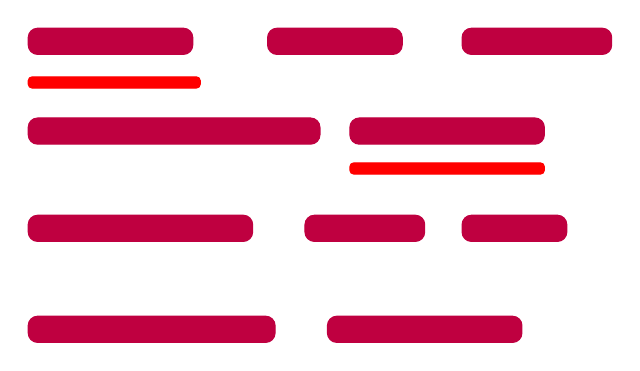
\begin{tikzpicture}[scale=0.95]
\draw[fill=purple, draw=purple, rounded corners=0.12cm] (-3.1,2.4) rectangle (-0.9,2.75);
\draw[fill=purple, draw=purple, rounded corners=0.12cm] (0.1,2.4) rectangle (1.9,2.75);
\draw[fill=purple, draw=purple, rounded corners=0.12cm] (2.7,2.4) rectangle (4.7,2.75);

\draw[fill=red, draw=red, rounded corners=0.05cm] (-3.1,1.95) rectangle (-0.8,2.1);

\draw[fill=purple, draw=purple, rounded corners=0.12cm] (-3.1,1.2) rectangle (0.8,1.55);
\draw[fill=purple, draw=purple, rounded corners=0.12cm] (1.2,1.2) rectangle (3.8,1.55);

\draw[fill=red, draw=red, rounded corners=0.05cm] (1.2,0.8) rectangle (3.8,0.95);

\draw[fill=purple, draw=purple, rounded corners=0.12cm] (-3.1,-0.1) rectangle (-0.1,0.25);
\draw[fill=purple, draw=purple, rounded corners=0.12cm] (0.6,-0.1) rectangle (2.2,0.25);
\draw[fill=purple, draw=purple, rounded corners=0.12cm] (2.7,-0.1) rectangle (4.1,0.25);

\draw[fill=purple, draw=purple, rounded corners=0.12cm] (-3.1,-1.45) rectangle (0.2,-1.1);
\draw[fill=purple, draw=purple, rounded corners=0.12cm] (0.9,-1.45) rectangle (3.5,-1.1);
\end{tikzpicture}
\end{figure}

The lecture then adds a second family of marks:
\begin{align}
\text{question mark} &\mapsto \text{highlight}, \\
\text{playful passage} &\mapsto \text{wavy underline}, \\
\text{aha moment} &\mapsto \text{black blob before it}, \\
\text{joke or funny story} &\mapsto \text{pink dots above it}.
\end{align}

These marks are not ornaments. They are instructions. They tell the voice what to do:
\begin{equation}
\text{script marks} \Longrightarrow \text{corresponding vocal changes}.
\end{equation}

\paragraph{Worked procedure.} The lecture's method may be written as a controlled passage from script to delivery.
\begin{enumerate}
\item Read the script sentence by sentence and underline the few words that carry the local burden.
\item Move up one scale and choose the single word in each paragraph that governs the paragraph's motion; underline it twice.
\item Mark questions, playful stretches, jokes, and the main aha moment with their own visual signals.
\item Read again, now letting pause, speed, softness, and emphasis respond to the marks.
\item Read once more, this time letting the emotional state of each section enter the voice.
\end{enumerate}

That final step prevents the whole procedure from becoming mechanical. The lecture explicitly asks us to remember the emotions attached to different parts of the talk: which passages arouse passion, anger, laughter, or confusion. Only then do the marks become more than typography. The check is empirical. We try it with a friend, or we record it and play it back with closed eyes.

\section{Body: Stance, Movement, and Stillness}

Only after the voice has been given a method does the lecture pivot to the body. Again it begins with a failure mode. Some speakers seem to arrive onstage with a body that exists only to carry the head. Once there, the body becomes uncertain: hands fixed at the sides, weight shifting, motion without intention.

The lecturer's first prescription is strikingly simple. Stand tall. Put equal weight on both feet. Keep the feet a few inches apart. The point is not theatrical grandeur. The point is a stable base from which the rest of the body can become legible.

\subsection{Question \& Answer}

\paragraph{Question.} Should a speaker stand still or move around the stage?

\paragraph{Answer.} Either can work. But stillness must be available, and movement must have purpose. The audience should see rhythm and control, not the outward leak of inner discomfort.

The visible slide gives us the key relation in symbolic form:
\begin{equation}
\text{weight on left foot} = \text{weight on right foot}.
\end{equation}

\begin{figure}[h]
\centering

\includegraphics[width=0.56\textwidth]{how_to_speak_with_meaning_figure_05.png}
\end{figure}

This equation is a cautious reconstruction. The equals sign is visible in the frame; the interpreted variables are supplied by the transcript. But the reconstruction is faithful to the lecture's point. Balance in the body is the first condition of calm power.

Once that base is stable, the upper body may move. Hands and arms may naturally emphasize what is being said. Good posture helps. Slouching weakens the signal. The lecture then broadens from stance to rhythm:
\begin{equation}
\text{purposeful movement} + \text{moments of stillness} \Longrightarrow \text{powerful stage rhythm}.
\end{equation}

The corresponding warning is equally sharp:
\begin{equation}
\text{constant pacing or rocking} \Longrightarrow \text{visible discomfort for the audience}.
\end{equation}

\paragraph{Practical rule.} The body-side algorithm of the lecture is short and concrete.
\begin{enumerate}
\item Establish a stable base.
\item Let gesture arise from the content rather than from anxiety.
\item Move when movement helps thinking or emphasis.
\item Stop when an important point needs to land.
\item Eliminate repetitive rocking, because it advertises nervousness more than meaning.
\end{enumerate}

The lecture's phrase ``calm power'' is apt here. We are not trying to freeze the body. We are trying to make it readable.

\section{No Single Style, Only Comfortable Confidence}

At this point the lecture makes an essential corrective move. After giving concrete rules of thumb, it refuses to turn them into a uniform model of good speaking. Some speakers sit for their talks. Some move with great energy. Some stand almost entirely still. The lecturer mentions Dame Stephanie Shirley, Oliver Sacks, and Clifford Stoll precisely to break the temptation toward imitation.

This is not a retreat from the earlier advice. It is its completion. The lecture's rules are not meant to manufacture sameness. They are meant to remove avoidable interference. Once that interference is gone, different stage styles can flourish without becoming distracting.

The final criterion is therefore not whether we resemble some canonical speaker. It is whether the way we occupy the stage makes us feel comfortable and confident, and whether it allows the idea to come through cleanly. The lecture keeps the test concrete: rehearse in front of a small audience, or watch yourself back, and ask whether your body language is helping or hindering the message.

This is also where the talk returns, quietly, to its opening logic. The whole purpose of delivery is to let the idea arrive with force. The body is not there to decorate the performance. It is part of the meaning-bearing apparatus.

\section{Summary}

The lecture unfolds as a controlled argument. We begin with a challenge: if the words already exist on the page, why speak them aloud at all? The answer is that live delivery adds a human layer that can turn information into inspiration. Once that is understood, the lecture reduces preparation to two variables we can actually work on: voice and body.

On the side of voice, the central principle is that variation must follow meaning. The voice should mark hierarchy, not flatten it. That is why the lecture gives us an explicit method for annotating the script: underline important words, double-mark the governing word of the paragraph, and add local signals for questions, playfulness, humor, and the main aha moment. On the side of body, the lecture begins with balance, then expands into gesture, movement, and stillness, always insisting that motion must serve emphasis rather than leak anxiety.

The chapter therefore ends where the lecture ends. There is no single performance style to imitate. What we want is a voice and a body that allow the idea to travel with clarity, conviction, and unmistakable human presence.